\documentclass[10pt]{article}
\usepackage{graphicx, url}
\setlength{\parskip}{1ex}
\setlength{\parindent}{0ex}
\begin{document}
\title{HDDM Design Specification}
\author{Richard Jones\\
University of Connecticut}
\date{September 21, 2003}
\maketitle
\vspace{2cm}
\begin{center}
request for comments, draft 1.1\\
updated from draft 1.0, May 25, 2001
\end{center}

\vspace{2cm}
\begin{abstract}
The GlueX experiment has adopted a policy that all shared data should
be described in xml.  A set of tools has been developed that enable
programmers to respect this policy without the overhead of having
to do building and parsing of xml documents in user code.  The data
are described in terms of data model structured like an xml document.
The general rules for building such model documents is called the
HDDM specification.  Once a user has described the data model in xml,
tools are provided to translate the model into c structures, xml
schema, and a general-purpose i/o library.
\end{abstract}

\newpage

\section{Background}
The workflow model for GlueX offline analysis is shown in Fig. 1.
It is important even at an early stage in the experiment to consider
carefully critical elements of the software framework in which these
components operate.  One critical aspect of the framework is the way
the data are represented at intermediate stages in the pipeline.  The
collaboration made an early decision to describe all such data in xml.
This choice brings with it the advantages of a host of automated tools
and libraries in the public domain for parsing and searching xml documents.
However it also demands careful design so that the additional software
layers introduced do not impose unintended restrictions on the client
programs.

A search on the web recently turned up a number of interesting projects
in which other groups are attempting to do the same or similar things.
Two projects stand out as most interesting from the point of view of
GlueX, the BinX project~\cite{binx} supported by the University of
Edinburgh and the HFS project~\cite{hdf} supported by NCSA, Urbana.

BinX is still in its infancy.  None of the tools or libraries described
in the reference document appear to be available for downloading at the
time of of this writing.  However from the description given, some
observations can be made.  The aim is to provide a general metadata format
for describing just about any binary data file.  The authors start from
the premise that storing and retrieving data files in xml format does not
make sense, and proceed to the conclusion that one never needs to actually
express them in xml.  Thus their goal appears to be to use the xml as a
sort of documentation facility that is separate from the actual process
of handling and interpreting the data.  This approach makes the most sense
when one is dealing with a set of i/o libraries and file formats that are
already in place, and wants to introduce a metadata description after the
fact.  In GlueX we have the possibility of starting out using the xml in
the design process, and having the other pieces automatically created from
the xml. BinX adds the metadata as a new layer on top of, and independent
from, the layer in which programs actually process data, and as such it
looks more like a retrofit tool than an integrated model component.
However it is still new and seems to have some resources behind it, so
GlueX developers should follow it with interest.

The Hierarchical Data Format HDF is much older, by contrast, and seems to
already have established a base of scientific users.  The design appears
to be oriented around the need to archive large multi-dimensioned arrays,
such as images.  Its origins date back to the mid-1990's before the advent
of xml and reflects that fact in the frequent references to storing and
recovering data from fortran programs, but it is being actively developed
and in version 5 (HDF5) they have included new functionality to describe
data in xml.  There are also java tools in the distribution, that probably
reflects the fact that support for scientific programming in java is on the
rise.  The primary concern regarding the potential usefulness of HFS to
GlueX is the complexity of the data model and the program interface.
This package is designed to do much more than is needed by GlueX.  For
example, the ability to delete arbitrary objects from existing data files,
or add new ones, complicates the i/o library considerably over what is
needed for HEP data streams.  The number of operations that are required
to set up a new data file are considerable, compared with the simple
opens and writes to which HEP programmers are accustomed.  From the point
of view of design, multi-dimensioned arrays are not the most appropriate
structure for expressing much of the content of a GlueX event.  While it
could probably be made to work for GlueX, it appears that HDF would be
overkill for this problem.  Thus there is still good reason to carry on
the earlier development of a xml data model for GlueX.

\begin{center}
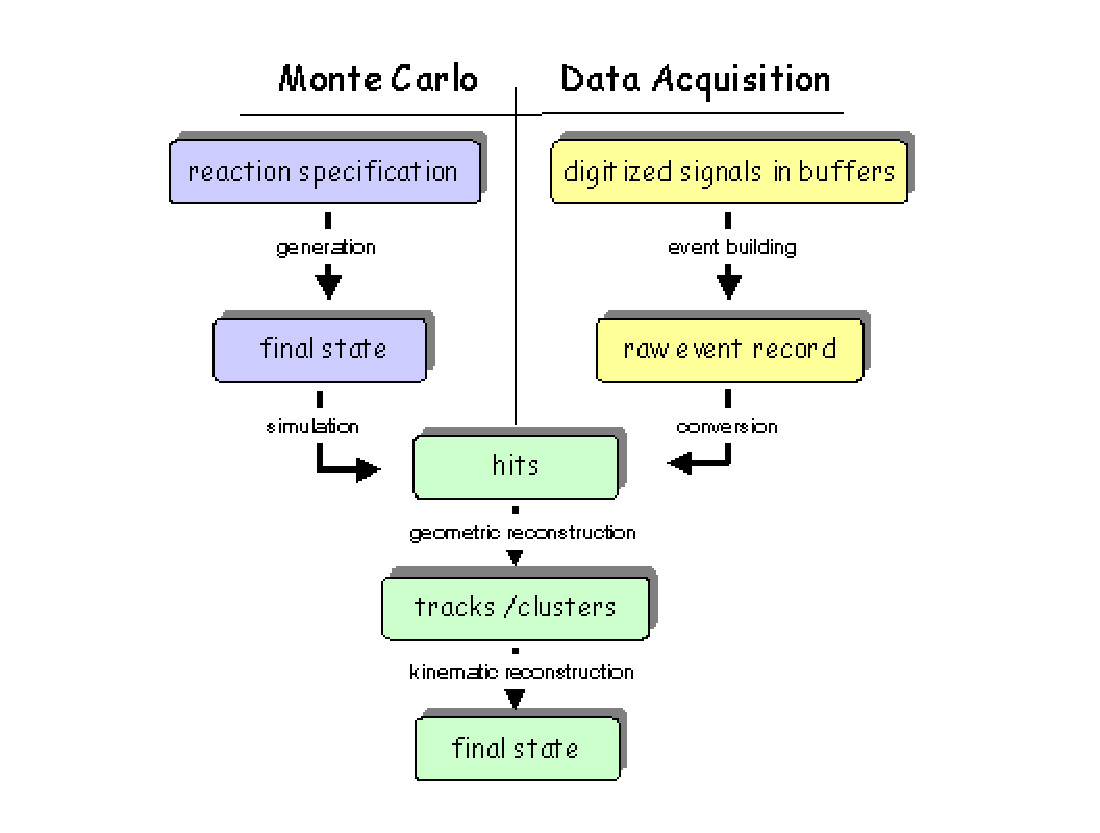
\includegraphics[scale=1]{./dataflow.eps} 
\end{center}
 Fig. 1: The conceptual data model for GlueX begins with a physics event, coming either from the detector or a Monte Carlo program, which builds up internal structure as it flows through the analysis pipeline. The data model specifies the elements of information that are contained in a view of the event at each stage and the relationships between them. The implementation provides standard methods for creating, storing and accessing the information. 


 
\section{General Notes}
\begin{enumerate}
\item  At each stage (lower-case items in diagram) in the pipeline one has a unique view of the event. 
\item  To each of these is associated a unique data model that expresses the event in that view. 
\item  GlueX policy is to use xml to describe all of our shared data, which means any data that might be passed as input to a program or produced as output. This does not mean that all data records are represented as plain-text files, but that to each data file or i/o port is attached some metadata that a tool can use to automatically express all of its contents in the form of a plain-text xml document. 
\item  This policy is interpreted to mean that to each data file or i/o port of a program is associated a xml schema that defines the data structure that the program expects or produces. The schemas should be either bundled with the distribution of the program, or published on the web and indicated by links in the Readme file. 
\item  Any xml document should be accepted as input to a program if it is valid according to the schema associated to that input port. 
\item  In practice, this last requirement adds significant of overhead to the task of writing a simple analysis program, because it must be capable of parsing general xml documents as input. In addition to this overhead imposed on the program code itself, the author must also produce schemas for each input or output port or file accessed by the program. 
\item  The purpose of the Hall D Data Model (HDDM) is to simplify the programmer's task by providing automatic ways to generate schemas and providing i/o libraries to standardize input and output of data in the form of xml-described files. 
\item  HDDM consists of a \emph{specification}
 supported by a \emph{set of tools}
 to assist its implementation. The \emph{specification}
 is a set of rules that a programmer must obey in constructing schemas in order for them to be supported by the tools. The \emph{tools}
 include an automatic schema generator and an i/o library builder for c and c++. 
\item  The HDDM specification was designed to enable the construction of an efficient i/o library. It was assumed in the design that users could not afford a general xml-parsing cycle every time an event is read in or written out by a program. It was also assumed that serializing data in plain-text xml is too expensive in terms of bandwidth and storage. Using the HDDM tools, users can efficiently pass data between programs in a serialized binary stream, and convert to/from plain-text xml representations using a translation tool when desired. 
\item  Programmers are not obligated to use HDDM tools to work in the GlueX software framework. If they provide their own schema for each file or i/o port used by the program and accept any xml that respects their input schema then they are within the agreed framework. 
\item  The HDDM tools are presently implemented in c and c++, so programmers wishing to work in java have more work to do. However, they will find it easy to interface to other programs that do use the HDDM libraries because they provide for the correct reading and writing of valid xml files and the automatic generation of schemas that describe them. 
\item  The \textbf{hddm-c}
 tool automatically constructs a set of c-structures based on xml metadata that can be used to express the data in memory. It also builds an i/o library that can be called by user code to serialize/deserialize these structures. 
\item  The serialized data format supported by \textbf{hddm-c}
 consists of a xml header in plain text that describes the structure and contents of the file, followed by a byte string that is a reasonably compact serialization of the structured data in binary form. Such \textbf{hddm}
 files are inherently self-describing. The overhead of including the metadata in the stream with the data is negligible. 
\item  The \textbf{hddm-xml}
 tool extracts the xml metadata from a hddm file header and expresses the data stored in the file in the form of a plain-text xml document. 
\item  The \textbf{hddm-schema}
 tool extracts the xml metadata from a hddm file header and generates a schema that describes the structure of the data in the file. The schema produced by \textbf{hddm-schema}
 will always validate the document produced by \textbf{hddm-xml}
 when both act on the same hddm file. More significantly, the schema can be used to check the validity of other xml data that originate from a different source. 
\item  The \textbf{xml-hddm}
 tool reads an xml document and examines its schema for compliance with the HDDM specification. If successful, it parses the xml file and converts it into hddm format. 
\item  The \textbf{schema-hddm}
 tool reads a schema and checks it for compliance with the HDDM specification. If successful, it parses it into the form of a hddm file consisting of the header only and no data. Such a data-less hddm file is also called a ``template'' (see below). 
\item  Note that the \textbf{hddm-xml}
, \textbf{hddm-schema}
, and \textbf{hddm-c}
 tools can act on any hddm data file written by any program, even if the code that produced the data is no longer available. This is because sufficient metadata is provided in the schema header to completely reconstruct the file's contents in xml, or instantiate it in c-structures. 
\item  A tool called \textbf{xml-xml}
 has been included in the tool set as a simple means to validate an arbitrary xml document against a dtd or schema, and reformat it with indentation to make it easier to read. 
\item  Tools called \textbf{stdhep2hddm}
 and \textbf{hddm2stdhep}
 provide conversion between the hddm data stream and the STDHEP format used by HDFast. This is an example where a user program achieves xml i/o by employing translators, in this case a two-stage pipeline. 
\item  In spite of the array of tools described above, the programmer still must do the work of describing the structure and contents of the data expected or produced by his program. He may do this in one of two ways: either he constructs an original schema describing his data, or he creates an original xml template of his data and then generates the schema using \textbf{hddm-schema}
. 
\item  Since schemas are rather verbose and repetitive, the suggested method is to create a template first, use \textbf{hddm-schema}
 to transform it into a basic HDDM schema, and then add facets to the schema to enrich the minimal set of metadata generated from the template. This method has the advantage that one starts off with a basic schema that is known to conform to the rules for HDDM schemas (see below) so it is relatively simple thereafter to stay within the specification. 
\item  As a shortcut to creating schemas, it is not necessary to do anything more than just create the template. The basic schema that is generated automatically from the template contains sufficient information to validate most data, so a programmer can get by without ever learning how to write or modify schemas. 

\end{enumerate}

\section{Rules for constructing HDDM templates}
\begin{enumerate}
\item  A hddm template is nothing more than a plain-text xml file that mimics the structure of the xml that the program expects on input or produces on output. In some ways it is like sample data that the programmer might provide to a user to demonstrate how to use it, although the comparison is not perfect. 
\item  The top element in the template must be $<$HDDM$>$ and have three required attributes: \emph{class}
, \emph{version}
, and \emph{xmlns}
. The value of the latter must be \emph{xmlns=''\url{http://www.gluex.org/hddm}''}
. The values of the class and version arguments are user-defined. They serve to identify a group of schemas that share a basic set of tags. See below for more details on classes. 
\item  The names of elements below the root $<$HDDM$>$ element are user-defined, but they must be constructed according to the following rules. 
\item  All values in hddm files are expressed as attributes of elements. Any text that appears between tags in the template is treated as a comment and ignored. 
\item  An element may have two information attached to it: child elements which appear as new tags enclosed between the open and close tags of the parent element, and attributes which appear as \emph{key=''value''}
 items inside the open tag. 
\item  All quantities in the data model are carried by named attributes of elements. The rest of the document exists to express the meaning of the data and the relationships between them. 
\item  All elements in the model document either hold attributes, contain other elements, or both. Empty elements are meaningless, and are not allowed. 
\item  One way a template is not like sample data is that it does not contain actual numerical or symbolic values for the fields in the structure. In the place of actual values, the types of the fields are given. For example, instead of showing \emph{energy=''12.5}
 as might be shown for sample data, the template would show in this position \emph{energy=''float''}
 or \emph{energy=''double''}
. 
\item  The complete list of allowed types supported by hddm is ``int'', ``long'', ``float'', ``double'', ``boolean'', ``string'', ``anyURI'', and ``Particle\_t''. The Particle\_t type is a value from an enumerated list of capitalized names of physical particles. The int type is a 32-bit signed integer, and long is a 64-bit signed integer. The other cases are obvious. 
\item  Attributes in the template that do not belong to this list are assumed to be constants. Constants are sometimes useful for annotating the xml record. The must have the same value for all instances of the element throughout the template. 
\item  Any given attribute may appear more than once throughout the template hierarchy. Wherever it appears, it must appear with identical attributes and with content elements of the same order and type. 
\item  Another difference between a template sample data is that the template never shows a given element more than once in a given context, even if the given tag would normally the repeated more than once for an actual sample. One obvious example of this is a physics event, which is represented only once in the template, but repeated multiple times in a file. 
\item  By default, it is assumed that an element appearing in the template must appear in that position exactly once. If the element is allowed to appear more than once or not at all then additional attributes should be inserted in the element of the form \emph{minOccurs=''N1''}
 and \emph{maxOccurs=''N2''}
, where \emph{N1}
 can be zero or any positive integer and \emph{N2}
 can be any integer no smaller than \emph{N1}
, or set to the string ``unbounded''. Each defaults to 1. 
\item  Arrays of simple types are represented by a sequence of elements, each carrying an attribute containing a single value from the array. This is more verbose than allowing users to include arrays as a simple space separated string of values, but the chosen method is more apt for expressing parallelism between related arrays of data. 
\item  An element may be used more than once in the model, but it may never appear as a descendent of itself. Such recursion is complicated to handle and it is hard to think of a situation where it is necessary. 
\item  Examples of valid hddm templates are given in the examples section below. 
\item  Because templates contain new tags that are invented by the programmer, it is not possible to write a standard template schema against which a programmer can check his new xml file for use as a template. Instead of using schema validation, the programmer can use the \emph{hddm-schema}
 tool to check a xml file for correctness as a hddm template. Any errors that occur in the hddm - schema transformation indicate problems in the xml file that must be fixed before it can be used as a template. 

\end{enumerate}

\section{Rules for constructing HDDM schemas}
\begin{enumerate}
\item  HDDM schemas must be valid xml schemas, belonging to the namespace \url{http://www.w3.org/2001/XMLSchema}. Not every valid schema is a valid HDDM schema, however, because xml allows for several different ways to express a given data structure. 
\item  GlueX programmers are not obligated to write schemas that conform to the HDDM specification, but if they do, they have the help of the HDDM tools for efficient file storage and i/o. 
\item  In the following specification, a prefix \emph{xs:}
 is applied to the names of elements, attributes or datatypes that belong to the official schema namespace ``\url{http://www.w3.org/2001/XMLSchema}'', whose meaning is defined by the xml schema standard. The extensions introduced for the specific needs of GlueX are assigned to a private namespace called ``\url{http://www.gluex.org/hddm}'' that is denoted by the prefix \emph{hddm:}
. 
\item  The top element defined by the schema must be $<$hddm:HDDM$>$ and have three required attributes: \emph{class}
, \emph{version}
, and \emph{xmlns}
. The value of the latter must be \emph{xmlns=''\url{http://www.gluex.org/hddm}''}
. The class and version arguments are of type \emph{xs:string}
 and are user-defined. They serve to identify a group of schemas that share a basic set of tags. See below for more details. 
\item  The names of elements below the root $<$hddm:HDDM$>$ element are user-defined, but they must be constructed according to the following rules. 
\item  An element may have two kinds of content: child elements and attributes, and hence must have \emph{xs:complexType}
. Elements represent the grouping together of related pieces of data in a hierarchy of nodes. The actual numerical or symbolic values of individual variables appear as the values of attributes. Examples are shown below. 
\item  All quantities in the data model are carried by named attributes of elements. The rest of the document exists to express the meaning of the data and the relationships between them. 
\item  All elements in the model document either hold attributes, contain other elements, or both. Empty nodes are meaningless, and are not allowed. 
\item  Text content between open and close tags is allowed in documents (\emph{type=''mixed''}
) but it is treated as a comment and stripped on translation. Basic HDDM schemas do not use \emph{type=''mixed''}
 elements. 
\item  The datatype of an attribute is restricted to a subset of basic types to simplify the task of translation. Currently the list is \emph{xs:int}
, \emph{xs:long}
, \emph{xs:float}
, \emph{xs:double}
, \emph{xs:boolean}
, \emph{xs:string}
, \emph{xs:anyURI}
 and \emph{hddm:Particle\_t}
. User types that are derived from the above by \emph{xs:restriction}
 may also be defined and used in a HDDM schema. 
\item  Attributes must always be either ``required'' or ``fixed''. Default attributes, i.e. those that are sometimes present inside their host and sometimes not are not allowed. This allows a single element to be treated as a fixed-length binary object on serialization, which has advantages for efficient i/o. 
\item  A datum that is sometimes absent can be expressed in the model by assigning it as an attribute to its own host element and putting the host element into its parent with \emph{minOccurs=''0''}
. 
\item  Fixed attributes (with \emph{use=''fixed''}
) may be attached to user-defined elements. They may be of any valid schema datatype, not just those listed above, and may be used as comments to qualify the information contained in the element. Because they have the same value for every instance of the element, they do not take up space in the binary stream, but they are included explicitly in the output produced by the \textbf{hddm-xml}
 translator. 
\item  All elements must be globally defined in the schema, i.e. declared at the top level of the \emph{xs:schema}
 element. Child elements are included in the definition of their parents through a \emph{ref=tagname}
 reference. Local definitions of elements inside other elements are not allowed. This guarantees that a given element has the same meaning and contents wherever it appears in the hierarchy. 
\item  Arrays of simple types are represented by a sequence of elements, each carrying an attribute containing a single value from the array. This is more verbose than allowing a simple list type like is defined by \emph{xs:list}
, but the chosen method is more apt for expressing parallelism between related arrays of data, such as frequently occurs in descriptions of physical events. Forbidding the use of simple \emph{xs:list}
 datatypes should encourage programmers to chose the better model, although of course they could just mimic the habitual use of lists by filling the data tree with long strings of monads! 
\item  Elements are included inside their parent elements within a \emph{xs:sequence}
 schema declaration. Each member of the sequence must be a reference to another element with a top-level definition. 
\item  A given element may occur only once in a given the sequence, but may have \emph{minOccurs}
 and \emph{maxOccurs}
 attributes to indicate possible absence or repetition of the element. 
\item  The \emph{sequence}
 is the only content organizer allowed by HDDM. More complex organizers are supported by schema standards, such as \emph{all}
 and \emph{choice}
, but their use would complicate the i/o i/o interfaces that have to handle them and they add little by way of flexibility to the model the way it is currently defined. 
\item  An element may be used more than once in the model, but it may never appear as a descendent of itself. Such recursion is complicated to handle and it is hard to think of a situation where it is necessary. 
\item  A user can check whether a given schema conforms to the HDDM rules by transforming it into a hddm template document. Any errors that occur during the transformation generate a message indicating where the specification has been violated. 

\end{enumerate}

\section{Class relationships between HDDM schemas}
\begin{enumerate}
\item  Two HDDM schemas belong to the same class if all tags that are defined in both have the same set of attributes in both. 
\item  This is a fairly weak condition. It is possible that all data files used in GlueX will belong to the same class, but it is not required. 
\item  If two HDDM schemas belong to the same class then it is possible to form a union schema that will validate documents of either type by taking the xml union of the two schema documents and changing any sequence elements in one and not in the other to \emph{minOccurs=''0''}
. 
\item  The translation tools \textbf{xml-hddm}
 and \textbf{hddm-xml}
 will work with any HDDM class. 
\item  Any program built using the i/o library created with \textbf{hddm-c}
 is dependent on the class of the schema used during the build. Any files it writes through this interface will be built on this schema, however it is able to read any file of the same class without recompilation. 
\item  A new schema may be derived from an existing HDDM schema by taking the existing one and adding new elements to the structure. In this case the version attribute of the HDDM tag should be incremented, while leaving the class attribute unchanged. 
\item  A program that was built using the \emph{hddm-c}
 tool for its i/o interface can read from any from any hddm file of the same class as the original schema used during the build. If the content of the file is a superset of the original schema then nothing has changed. If some elements of the original schema are missing in the file then the i/o still works transparently, but the c-structures corresponding to the missing elements will be empty, i.e. zeroed out. 
\item  The c/c++ i/o library rejects an attempt to read from a hddm file that has a schema of a different class from the one for which it was built. 
\item  No mandatory rules are enforced on the \emph{version}
 attribute of the hddm file, but it is available to programs and may be used to select certain actions based on the ``vintage'' of the data. 
\item  Programs that need simultaneous access to multiple classes of hddm files can be built with more than one i/o library. The structures and i/o interface are defined in separate header files hddm\_\emph{X}
.h and implementation files hddm\_\emph{X}
.c, where \emph{X}
 is the class letter. 

\end{enumerate}

\section{Implementation Notes}
\begin{enumerate}
\item  There is a complementarity between xml schemas and the xml templates that express the metadata in hddm files. Depending on the level of detail desired, schemas may become arbitrarily sophisticated and complex. On the other hand, only a small subset of that information is needed to support the functions of the hddm tool set. Templates allow that information to be distilled in a compact form that is both human-readable and valid xml. 
\item  In the present implementation, the text layout of the template (including the whitespace between the tags) is used by the hddm tools to simplify the encoding and decoding. There is exactly one tag per line and two leading spaces per level of indent. This may change in future implementations. This means that hddm file headers should not be edited by hand. 
\item  The XDR~\cite{xdr} library is used to encode the binary values in the hddm stream. This means that hddm files are machine-independent, and can be read and written on any machine without any dependence on whether the machine is little-endian or big-endian. XDR is the network encoding standard library developed for Sun's rpc and nfs services. For more info, search for RFC 1014 on the web or do ``man xdr'' under linux. 
\item  The binary file format will change. The point is not to fix on some absolute binary format at this early stage. The only design constraint was that the data model be specified in xml and that the data be readily converted into plain-text xml, preferably without needing to look up auxiliary files or loading the libraries that wrote it. 
\item  The design of the i/o library has been optimized for flexibility: the user can request only the part of the model that is of interest. The entire model does not even have to be present in the file, in which case only the parts of the tree that are present in the file are loaded into memory, and the rest of the requested structure is zeroed out. 
\item  The only constraint between the model used in the program and that of the hddm stream is that there be no collisions, that is tags found in both but with different attributes. 
\item  Two data models with colliding definitions can be used in one program but they have to have different class Ids. Two streams with different class Ids cannot feed into each other. In any case the xml viewing tool \emph{hddm-xml}
 can read a hddm stream of any class. 

\end{enumerate}

\section{Examples}
\begin{enumerate}
\item  A simple model of an event fragment describing hits in a time-of-flight wall. It allows for multiple hits per detector in a single event, with \emph{t}
 and \emph{dE}
 information for each hit. The hits are ordered by side (right: end=0, left: end=1) and then by horizontal slab. The minOccurs and maxOccurs attributes allow those tags to appear any number of times, or not at all, in the given context. \begin{verbatim}

<forwardTOF>
  <slab y="float" minOccurs="0" maxOccurs="unbounded">
    <side end="int" minOccurs="0" maxOccurs="unbounded">
      <hit t="float" dE="float" maxOccurs="unbounded" />
    </side>
  </slab>
</forwardTOF>

\end{verbatim}

\item  A model of the output from an event generator. An example of actual output from genr8 converted to xml using hddm-xml. Warning: some browsers have difficulty displaying plain xml. Mozilla 1.x and Internet Explorer 6 give a nice view of the document below. \begin{verbatim}

<?xml version="1.0" encoding="UTF-8"?>

<HDDM class="s" version="1.0" xmlns="http://www.gluex.org/hddm">
  <physicsEvent eventNo="int" runNo="int">
    <reaction type="int" weight="float" maxOccurs="unbounded">
      <beam type="Particle_t">
        <momentum px="float" py="float" pz="float" E="float" />
        <properties charge="int" mass="float" />
      </beam>
      <target type="Particle_t">
        <momentum px="float" py="float" pz="float" E="float" />
        <properties charge="int" mass="float" />
      </target>
      <vertex maxOccurs="unbounded">
        <product type="Particle_t" decayVertex="int" maxOccurs="unbounded">
          <momentum px="float" py="float" pz="float" E="float" />
          <properties charge="int" mass="float" />
        </product>
        <origin vx="float" vy="float" vz="float" t="float" />
      </vertex>
    </reaction>
  </physicsEvent>
</HDDM>

\end{verbatim}

\item  A more complex example follows, showing a hits tree for the full detector. \begin{verbatim}

<?xml version="1.0" encoding="UTF-8"?>

<HDDM class="s" version="1.0" xmlns="http://www.gluex.org/hddm">
  <physicsEvent eventNo="int" runNo="int">

    <hitView version="1.0">
      <barrelDC>
        <cathodeCyl radius="float" minOccurs="0" maxOccurs="unbounded">
          <strip sector="int" z="float" minOccurs="0" maxOccurs="unbounded">
            <hit t="float" dE="float" maxOccurs="unbounded" />
          </strip>
        </cathodeCyl>
        <ring radius="float" minOccurs="0" maxOccurs="unbounded">
          <straw phim="float" minOccurs="0" maxOccurs="unbounded">
            <hit t="float" dE="float" minOccurs="0" maxOccurs="unbounded" />
            <point z="float" dEdx="float" phi="float"
                        dradius="float" maxOccurs="unbounded" />
          </straw>
        </ring>
      </barrelDC>
    
      <forwardDC>
        <package pack="int" minOccurs="0" maxOccurs="unbounded">
          <chamber module="int" minOccurs="0" maxOccurs="unbounded">
            <cathodePlane layer="int" u="float" minOccurs="0" maxOccurs="unbounded">
              <hit t="float" dE="float" minOccurs="0" maxOccurs="unbounded"/>
              <cross v="float" z="float" tau="float" maxOccurs="unbounded" />
            </cathodePlane>
          </chamber>
        </package>
      </forwardDC>
    
      <startCntr>
        <sector sector="float" minOccurs="0" maxOccurs="unbounded">
          <hit t="float" dE="float" maxOccurs="unbounded" />
        </sector>
      </startCntr>
    
      <barrelCal>
        <module sector="float" minOccurs="0" maxOccurs="unbounded">
          <flash t="float" pe="float" maxOccurs="unbounded" />
        </module>
      </barrelCal>
        
      <Cerenkov>
        <module sector="float" minOccurs="0" maxOccurs="unbounded">
          <flash t="float" pe="float" maxOccurs="unbounded" />
        </module>
      </Cerenkov>
    
      <forwardTOF>
        <slab y="float" minOccurs="0" maxOccurs="unbounded">
          <side end="int" minOccurs="0" maxOccurs="unbounded">
            <hit t="float" dE="float" maxOccurs="unbounded" />
          </side>
        </slab>
      </forwardTOF>
    
      <forwardEMcal>
        <row row="int" minOccurs="0" maxOccurs="unbounded">
          <column col="int" minOccurs="0" maxOccurs="unbounded">
            <flash t="float" pe="float" maxOccurs="unbounded" />
          </column>
        </row>
      </forwardEMcal>
    </hitView>
  </physicsEvent>
</HDDM>

\end{verbatim}
\end{enumerate}

\begin{thebibliography}{d}
\bibitem{binx}
``Representing Scientific Data on the Grid with BinX, Binary XML Description
Language'', M. Westhead and M. Bull, University of Edinburgh, January 2003.
\tt{"http://www.epcc.ed.ac.uk/~gridserve/WP5/Binx/sci-data-with-binx.pdf"}
\bibitem{hdf}
``HDF5 Users's Guide'', working draft, July 2003.
\tt{http://hdf.ncsa.uiuc.edu/HDF5/doc/UG/}
\bibitem{xdr}
``RFC 1832 (rfc1832) - XDR: External Data Representation standard'',
September 1995.
\tt{http://www.faqs.org/rfcs/rfc1832.html}
\end{thebibliography}

This material is based upon work supported by the National Science Foundation under Grant No. 0072416. 

\end{document}
